\chapter{Experimental Setup}
\label{chap:experimental_setup}

In the following, we outline the experimental setup for the experiments we ran.
This includes not only allocation, preprocessing and pair selection of each dataset, but also a description and motivation for the experiments carried out.


\section{Dataset}
\label{sec:dataset}

Since our method extends the original \impAppr{} proposed by \citet{koppel_determining_2014}, we first obtained the datasets used in their study to validate our implementation and reproduce their results. 
The original experiments were conducted on the \dataBlog{} and \dataStudent{} datasets, which are described in detail in \autoref{subsec:original_data}. 
In addition to these, we incorporated two supplementary datasets, \dataPan{} and \dataGutenberg{}, presented in \autoref{subsec:additional_data}. 
Following the general description of all datasets, we outline our preprocessing pipeline in \autoref{subsec:dataset_preprocessing} and conclude with the text-pair selection procedure in \autoref{subsec:dataset_text_pair_selection}.


\subsection{Original Data}
\label{subsec:original_data}

% Blog
The \dataBlog{} corpus~\citep{blog_dataset_2006} consists of blog posts collected from \textit{blogger.com} on or before August 2004, with each blog authored by a single user.
According to the Kaggle repository~\footnote{\href{https://www.kaggle.com/datasets/rtatman/blog-authorship-corpus?resource=download}{Kaggle dataset \texttt{rtatman/blog-authorship-corpus}} (26.07.2025)}, the dataset contains \num{681288} posts from \num{19320} bloggers, averaging approximately 35 posts and \num{7250} words per author.
Users are grouped into three age categories: 13-17, 23-27, and 33-47.
Each record includes the following metadata: \texttt{id}, \texttt{gender}, \texttt{age}, \texttt{topic}, 
\texttt{sign} (referring to the author's astrological/zodiac sign), \texttt{date}, and \texttt{text}.

% student essays
The \dataStudent{} dataset is not publicly available due to the presence of sensitive student information. 
We gratefully acknowledge J. W. Pennebaker for granting access to the original data used by \citet{koppel_determining_2014} in their study. 
The dataset comprises \num{7052} student essays written for five assignments by a cohort of 950 university students in 2006~\citep{koppel_determining_2014}.

The assignments include (1) a stream-of-consciousness task, (2) a reflections on childhood, (3) a self-assessment of personality, (4) a thematic apperception test, and (5) four examples of four different theories.
An inconsistency in the file naming convention is notable: 
Most files are named solely by the author ID, whereas those from the first assignment follow the format \texttt{2006\_authorID}.
Following \citet{koppel_determining_2014}, our \impAppr{} experiments employ only the first four assignments. 
Consistent with \citet{koppel_determining_2014}, disputed–candidate pairs in our setup are drawn from different assignments, irrespective of their class label (\texttt{same-author} or \texttt{different-author}).
In contrast to the original \impAppr{}, which truncated each essay to the first 500 words, we crop texts to the minimum length of the text pair.

Due to privacy restrictions, researchers seeking access to the \dataStudent{} dataset should contact J. W. Pennebaker, the official data custodian. 
For establishing a baseline in our \imp{} experiments, we use both the \dataBlog{} and \dataStudent{} datasets.


\subsection{Additional Data}
\label{subsec:additional_data}
To broaden the evaluation scope of the \impAppr{}, we incorporated additional datasets selected according to two criteria:
(1) control over confounding factors such as genre and topic, and 
(2) verified, undisputed authorship.
Both the \dataPan{} and \dataGutenberg{} datasets satisfy these conditions.

% PAN20: Fanfiction
The \dataPan{} corpus~\citep{bischoff_importance_2020} comprises fanfiction texts sourced from \textit{fanfiction.net}.
Each text belongs exclusively to one fandom (i.e. thematic category), with no crossovers between fandoms.
According to \href{https://pan.webis.de/clef20/pan20-web/author-identification.html}{the official \ac{pan} website}, 
train and test set originate from two different fanfictions and approximate the (long-tail) distribution of the fandoms in the original dataset.
Dataset features include \texttt{id}, \texttt{fandoms}, and \texttt{pair}, where the latter contains the paired texts.
An additional \texttt{jsonl} file provides the ground truth for each pair, specifying \texttt{id}, \texttt{same} (authorship label), and \texttt{authors}.

% Gutenberg
The \dataGutenberg{} dataset~\footnote{\href{https://www.gutenberg.org/}{Project Gutenberg} (26.07.2025)} contains a curated selection of literary works from Project Gutenberg, a digital library dedicated primarily to older works whose U.S. copyrights have expired.
As of this writing, the collection contains over \num{75000} digitized and proofread e-books contributed by volunteers.
For our experiments, we selected 19 works authored by 7 writers from the 16th to 19th centuries, covering genres such as drama, fiction, and poetry.
Metadata for these works was manually extracted from the Project Gutenberg website and Wikipedia.


\subsection{Dataset Preprocessing}
\label{subsec:dataset_preprocessing}

To control confounding factors that influence authorial style, we preprocess each dataset twice:
(1) Prior to generating arrow dataset file and (2) before using the \impAppr{}.
This two-stage approach addresses both experimental scenarios, where all material is prepared in advance, and inference scenarios in which the \impAppr{} model is applied directly to texts.
The preprocessing process was designed to meet the following requirements:
\begin{itemize}
    \item Removal of all formatting and layout information to produce plain text.
    \item Cropping texts to match the length of the shorter text in each pair.
\end{itemize}
It is important to note that text-length adjustment is performed exclusively within the \impAppr{} implementation and is not applied to the Arrow dataset itself.
For a controlled evaluation environment in our \impAppr{}, we opted to work with relatively small, curated datasets rather than scaling to larger collections.  
The effect of individual preprocessing steps on vocabulary size was analysed, with results presented in \autoref{fig:preprocesing_impact_vocab_size}.
In line with \citep{koppel_determining_2014}, the vocabulary consists of space-free character 4-grams.
Removing formatting and layout information includes removing HTML artefacts, play artefacts, newlines, 
converting UTF-8 to ASCII, and stripping leading and trailing whitespace.
Since both \dataBlog{} and \dataPan{} originate from the Internet, we applied HTML-specific preprocessing steps, which had minimal impact on their respective vocabularies.
Upon inspection of the \dataGutenberg{}, we found that certain patterns reappear due to the \textit{play} genre. 
Notably, since we do not consider actor instructions (e.g., character cues) or structural elements (e.g., chapter headings) as part of authorial style, these patterns were removed using regular expressions.
We opted to forgo lowercasing the texts, as our preliminary analysis indicated that lowercasing had no meaningful effect on any dataset while potentially discarding deliberate authorial capitalization choices.

\begin{figure}[htbp]
    \centering
    \includesvg[width=\textwidth]{images/dataset/impact_preprocessing_steps.svg}
    \caption{Effect of preprocessing steps on vocabulary size (space-free character 4-grams).}
    \label{fig:preprocesing_impact_vocab_size}
\end{figure}


\subsection{Selection of Text Pairs}
\label{subsec:dataset_text_pair_selection}

For the \dataBlog{}, \dataStudent{}, and \dataGutenberg{} datasets, we selected pairs of texts according to specific criteria to control potential confounding factors.
Only texts with a minimum length of \num{700} words were considered eligible. 
For the \dataPan{} dataset, we retained the existing pairs in the Arrow dataset to ensure comparability with prior work. 
All datasets include both same-author and different-author pairs. 

For \dataBlog{}, pairs were constructed so that the two texts share the same topic, year, gender, and age (the latter referencing the author). 
The training set comprises 80\% of the data and the test set 20\%, with different topics assigned to each split.

For \dataStudent{}, texts were assigned to either the training (70\%) or test (30\%) set. 
The test set is larger because each author typically contributes only one essay per task and if only a single task were included in the test set, no same-author pairs could be formed. 
Same-author pairs were selected such that authors share the same sex, ethnicity, and political orientation. 
As per \citep{koppel_determining_2014}, all text pairs are drawn from the different tasks.



% Please add the following required packages to your document preamble:
% \usepackage{graphicx}
\begin{table}[tbp]
    \centering
    \caption{\ac{aa} scenarios with author $i$ is shortened with $A_i$ \citep{altakrori_topic_2021}.}
    \label{tab:aa_same_topic}
    \begin{tabular}{|l|l|l|}
    \hline
    \textbf{} & \textbf{Train} & \textbf{Test} \\ \hline
    \textbf{Topic $T_1$} & $A_1, A_2$ & $A_1, A_2$ \\ \hline
    \textbf{Topic $T_2$} & $A_1, A_2$ & $A_1, A_2$ \\ \hline
    \end{tabular}%
\end{table}

% Please add the following required packages to your document preamble:
% \usepackage{graphicx}
\begin{table}[tbp]
    \centering
    \caption{\ac{aa} scenarios with author $i$ is shortened with $A_i$ \citep{altakrori_topic_2021}.}
    \label{tab:aa_cross_topic}
    \begin{tabular}{|l|l|l|}
    \hline
    \textbf{} & \textbf{Train} & \textbf{Test} \\ \hline
    \textbf{Topic $T_1$} & $A_1, A_2$ &  \\ \hline
    \textbf{Topic $T_2$} &  & $A_1, A_2$ \\ \hline
    \end{tabular}%
\end{table}

% Please add the following required packages to your document preamble:
% \usepackage{graphicx}
\begin{table}[tbp]
    \centering
    \caption{\ac{aa} scenarios with author $i$ is shortened with $A_i$ \citep{altakrori_topic_2021}.}
    \label{tab:aa_topic_confusion}
    \begin{tabular}{|l|l|l|}
    \hline
    \textbf{} & \textbf{Train} & \textbf{Test} \\ \hline
    \textbf{Topic $T_1$} & $A_1$ & $A_2$ \\ \hline
    \textbf{Topic $T_2$} & $A_2$ & $A_1$ \\ \hline
    \end{tabular}%
\end{table}


For the \dataGutenberg{} dataset, pairs were selected such that texts share the same genre and century. 
Authors were split into training (80\%) and test (20\%) sets.

Regardless of the selection criteria, the final datasets contain only three columns: \texttt{authors}, \texttt{pair}, and \texttt{same}.
The \texttt{pair} column contains the texts of the pair as a list of strings,
the \texttt{authors} column contains the authors of the texts as a list of strings,
and the \texttt{same} column indicates whether the texts are from the same author (\texttt{True}) or from different authors (\texttt{False}).
Descriptive statistics for all preprocessed datasets are provided in Table~\ref{tab:data_stats}.

% minimum length necessesary for AV/ AA
The choice of minimum text length was informed by related research in \ac{av} and \ac{aa}.
\citet{bevendorff_generalizing_2019}used text chunks of at least 700 words for an unmasking approach, while \citet{koppel_authorship_2004} set the minimum at 500 words.
Recent work~\citep{llm_detection_av_2025} identifies \num{2500}-\num{4000} characters to be sufficient for effective \ac{llm} detection framed as \ac{av} or \ac{aa}, leading those authors to adopt a \num{3000}-character minimum for their datasets.

% \begin{table}[h]
\begin{sidewaystable}
\centering\small
\caption{Statistics of preprocessed datasets \dataPan{}, \dataBlog{}, \dataGutenberg{}, and \dataStudent{}.}
\label{tab:data_stats}
\resizebox{\textwidth}{!}{%
\begin{tabular}{@{}lrrrrrrrrr@{}}   % numbers should be right aligned, text left aligned
\toprule
dataset & num\_pairs & num\_authors & num\_same\_pairs & num\_different\_pairs & avg\_text\_len & max\_text\_len\_words & std\_text\_len\_words & median\_text\_len\_words \\
\midrule
pan20           & 66905 & 52771 & 35616 & 31289 & 21418.76 (3914.76)   & 55413 & 512.19 & 3889 \\
blog            & 11565 & 5997  & 6204 & 5361  & 6249.94 (1154.25)     & 115365 & 1493.97 & 913 \\
gutenberg       & 12    & 7     & 6     & 6     & 437870.75 (78698.79) & 297704 & 68329.91 & 60282 \\
student\_essays & 224  & 222   & 112   & 112  & 4459.32 (865.90)     & 1634 & 157.41 & 815  \\
\bottomrule
\end{tabular}%
}
% \end{table}
\end{sidewaystable}


% regardless of experimental design
\section{Evaluation measures}
\label{sec:evaluation_measures}

In this chapter, we introduce state-of-the-art quantitative evaluation metrics for \ac{aa}, \ac{av}, and paraphrase generation. 
Unlike subjective human judgments, these metrics are designed to be comparable and reproducible, providing a more objective basis for evaluation.

\textcolor{red}{
c@1 does not make sense here bc (1) output is "same author" or "i do not know" (standard 0.5 from PAN) and (2) output is 0 or 1, that is why we have threshold -> never 0.5. Maybe we could train two thresholds and could return 0.5 if neither is triggered, but does not make sense bc "different author" class ill-defined (open set -> no representative/exhaustive samples)
}


We will present state-of-the-art quantitative evaluation measures for \ac{aa}, \ac{av} and paraphrase generation.
Ideally, quantitative measures are comparable and reproducible since they do not arise from human biased judgment.

\section{\ac{av} Quality Measures}
\label{sec:av_quality_measures}

Common metrics for evaluating the \ac{av} performance are:
\begin{itemize}
    \item $Accuracy = \frac{TP + TN}{TP + TN + FP + FN}$ \citep{elmanarelbouanani_authorship_2014,neal_surveying_2018} 
    measures the percentage of classified correctly over all test cases \citep{neal_surveying_2018}.

    \item $Precision = \frac{TP}{TP + FP}$ \citep{elmanarelbouanani_authorship_2014,neal_surveying_2018,chen_web_2008} 
    measures how often a system gets positive classification correctly \citep{neal_surveying_2018}.

    \item $Recall = \frac{TP}{TP + FN}$ \citep{elmanarelbouanani_authorship_2014,neal_surveying_2018,chen_web_2008} 
    measures how often a system correctly classifies positive samples when it encounters them \citep{neal_surveying_2018}.
    Recall is also called sensitivity or \acl{tp} rate \citep{palivela_optimization_2021}

    \item $F-measure = \frac{2 \cdot precision \cdot recall}{precision + recall}$~\citep{chen_web_2008,abbasi_writeprints_2008}

    % PAN
    \item \ac{roc-auc} \citep{bevendorff_overview_2024,weerasinghe_feature_vector_difference_2021,kocher_unine_2015}
    where \ac{roc} plots \ac{fpr} $= \frac{FP}{FP+TN}$ on the x-axis against the \ac{tpr} $=\frac{TP}{TP+FN}$ on the y-axis 
    for varying thresholds \citep{kocher_unine_2015,neal_surveying_2018}.
    The maximum \ac{roc} value of 1.0 indicated a perfect performance \citep{kocher_unine_2015}.
    Greater \ac{auc} indicates a better performance \citep{neal_surveying_2018}.
    % The \ac{auc} of the \ac{roc} is biased since the \ac{roc} gives more emphasis 
    % on the first position and therefore increases the total \ac{auc}.
    % A misclassification with a lower probability is less penalized with \ac{roc-auc} \citep{kocher_unine_2015}.
    \citet{kocher_unine_2015} claim that both \ac{roc} and \ac{auc} are difficult to interpret.
    % LLM detection as AV task
    \citet{llm_detection_av_2025} argue that the reduction from the \ac{fpr}-\ac{tpr} curve of \ac{roc} to a single \ac{roc-auc} number 
    comes with information loss due to the absence of a fixed threshold and trade-off.
    Moreover, \ac{roc}'s \ac{fpr} and \ac{tpr} are independent of class prevalence, which is desirable.
    However, in highly imbalanced class scenarios \ac{roc} can be misleading (overly optimistic or pessimistic).
    
    \item BRIER: Complement of the Brier score \citep{bevendorff_overview_2024,weerasinghe_feature_vector_difference_2021}, 
    in \citet{bevendorff_overview_2024}'s case equivalent to the mean squared loss.
    The Brier score is used to evaluate the ability of \ac{av} methods to abstain from hard samples \citep{tyo_state_2022}.
    
    \item $C@1 = \frac{nc}{np}(1+\frac{nu}{np})$ where $np$ is the number of problems, $nc$ the number of correct answers, 
    and $nu$ the number of unanswered problems \citep{kocher_unine_2015}. 
    Modified version of the accuracy \citep{bevendorff_overview_2024}/ F1-score \citep{weerasinghe_feature_vector_difference_2021} score, 
    where the non-answers (abstained) \citep{llm_detection_av_2025} are assigned the average accuracy of the remaining cases \citep{bevendorff_overview_2024}. 
    It rewards systems that leave difficult problems unanswered \citep{weerasinghe_feature_vector_difference_2021}.
    
    \item $F_1 = 2 \cdot \frac{precision \cdot recall}{precision + recall}$~\citep{neal_surveying_2018}: Harmonic mean of precision and recall \citep{bevendorff_overview_2024,weerasinghe_feature_vector_difference_2021}.
    A higher value indicates a better performance \citep{neal_surveying_2018}.
    
    \item $F_{0.5u}$: Modified version of the $F_{0.5}$ score, where the non-answers are considered \acp{fn} \citep{bevendorff_overview_2024}. 
    A measure that puts more emphasis on deciding same-author cases correctly \citep{weerasinghe_feature_vector_difference_2021}.
    Used to evaluate the ability of \ac{av} methods to abstain from hard samples \citep{tyo_state_2022}.
\end{itemize}
$TP$ is the number of \aclp{tp}, $FP$ is the number of \aclp{fp} 
and $FN$ is the number of \aclp{fn}~\citep{chen_web_2008}.



% PAN AA & AV metrics: Abstaining from hard samples
% The \todo{F0.5u, C@1, and Brier Score metrics} are used to evaluate the ability of \ac{av} methods 
% to abstain from hard samples \citep{tyo_state_2022}.
% For each sample, a score $\in [0, 1]$ is assigned to the sample.
% A score of exactly 0.5 means the model abstains from the sample \citep{tyo_state_2022,bevendorff_overview_2024,kocher_unine_2015}.

% The AUC metric is used to evaluate the ability of methods to rank predictions.
% No threshold is required.
% \ac{pan} ignores any abstained samples when calculating the AUC metric \citep{tyo_state_2022}.

% != PAN
% \citet{tyo_state_2022} chose to adopt the macro-averaged accuracy metric, so-called macro-accuracy, for \ac{aa}, 
% and AUC \ac{av} tasks.

\subsection{Paraphrase evaluation}
\label{subsec:paraphrase_evaluation}

Evaluating paraphrases is a central problem in \ac{nlp}, yet it is complicated by the fact that there is no universal definition of what constitutes a paraphrase. 
Definitions vary in degree of semantic equivalence required. 
This conceptual ambiguity makes the task of evaluation especially challenging, since different applications may prioritize different aspects such as fidelity to meaning, stylistic variation, or grammatical well-formedness.

Because of this, paraphrase evaluation cannot be reduced to syntactic variance alone. 
A meaningful assessment must account both for syntactic diversity and for the extent to which semantic content is preserved. 
At the same time, paraphrases must be judged for their fluency and acceptability, as grammatical errors or stylistic awkwardness may render an otherwise accurate reformulation unsuitable in practice.

Existing approaches can broadly be grouped into automatic and human-based methods. 
Automatic measures attempt to quantify the similarity or equivalence between a candidate and a reference paraphrase using algorithmic techniques. 
These methods can be further distinguished by the linguistic level at which they operate. 
Some focus on syntactic structure and word overlap, while others rely on semantic representations to evaluate meaning preservation beyond surface form. 
Human evaluation, in contrast, remains the gold standard, as it incorporates judgments about adequacy, grammaticality, and contextual appropriateness that automatic measures cannot fully capture.

% Syntactic (\ac{bleu}, \ac{rouge}-1, \ac{rouge}-L), semantic (BERTScore, cosine similarity of SBERT vectors, WMS), human evaluation (TODO)

% There is manual (by humans) evaluation and automatic evaluation for paraphrase generation \citep{fu_learning_2024,zhou_paraphrase_2021}.
% According to \citet{zhou_paraphrase_2021}, automatic evaluation metrics mainly focus on the n-gram overlaps instead of meaning, 
% and hence, human evaluation is more accurate and has a higher quality.
% In the following, we focus on automatic evaluation.

In the following, we examine both automatic and human evaluation strategies. 
The automatic measures are divided into syntactic and semantic approaches, reflecting the different dimensions along which paraphrases can be compared. 
This is followed by a discussion of human evaluation, which complements automatic measures by providing a more comprehensive assessment of paraphrase quality.


\subsection{Traditional Quantitative Paraphrase Evaluation Measures}
\label{subsec:traditional_quantitative_evaluation_measures}

Evaluating paraphrases can be reduced to summarization or translation evaluation.
The evaluation of paraphrases can be divided into syntactic and semantic approaches. 
% \citet{gohsen_captions_2023} normalized all metrics and averaged the semantic and syntactic scores separately.

\subsubsection{Syntactic Measures}
Syntactic evaluation metrics mainly focus on the n-gram overlaps~\citep{zhou_paraphrase_2021}. 
Common syntactic evaluation metrics include \acs{bleu}, \acs{rouge}-1, and \acs{rouge}-L.

\paragraph{\ac{bleu}}
\ac{bleu}~\citep{papineni_bleu_2001} was originally developed for machine translation~\citep{zhou_paraphrase_2021,anantha_pearson_metrics_2021}. 
\ac{bleu}'s basic unit of evaluation is a sentence. 
\ac{bleu} is based on precision, i.e.\ computing the fraction of generated word n-grams $n\text{-}gram \in \mathcal{C}$ that appear in any reference text $r$~\citep{kurt_pehlivanoglu_comparative_2024,palivela_optimization_2021,papineni_bleu_2001,anantha_pearson_metrics_2021}. 
In our case, there is only one reference.
We consider the reference the ground truth text.
To prevent inflated precision scores $p_n$ due to repetition of frequent tokens (e.g.\ "the"), \ac{bleu} introduces a clipping mechanism $\operatorname{Count_{match}}(.)$ that caps n-gram counts at their maximum reference frequency~\citep{papineni_bleu_2001}. 
Precision $p_n$ for $n \in \mathbb{N}_{>0}$ is given by \Cref{eq:bleu}.

\begin{equation}
    p_n = \sum_{\mathcal{C} \in \left\{ Candidates \right\}}\sum_{n\text{-}gram \in\mathcal{C}} \frac{\operatorname{Count_{match}}(n\text{-}gram)}{\operatorname{Count}(n\text{-}gram)}
\label{eq:bleu}
\end{equation}

The choice of $n$ determines what syntactic characteristic is evaluated.
Uni-grams are used to test adequacy, while longer n-grams are used to test fluency~\citep{papineni_bleu_2001}. 
The brevity penalty $\operatorname{BP}$ from \Cref{eq:bleu_brevity_penalty} is applied to discourage excessively short candidates $c$~\citep{papineni_bleu_2001}.

\begin{equation}
    \operatorname{BP} = \begin{cases}
        1 & \text{if } \operatorname{len}(c) > \operatorname{len}(r) \\
        e^{1 - \frac{r}{c}} & \text{else}
    \end{cases}
\label{eq:bleu_brevity_penalty}
\end{equation}

In order to compute the \ac{bleu} score from \Cref{eq:bleu} for more than one sentence, 
one (1) computes the clipped n-gram matches sentence by sentence, 
then (2) adds them across all sentences, 
and finally (3) divides the total clipped n-gram matches by 
the total number of unclipped n-grams in all candidate sentences~\citep{papineni_bleu_2001,cordeiro_bleu_2007}.

Combined scores across different n-gram orders are computed via the geometric mean, weighted uniformly (i.e.\ $w_n$) across different $n$~\citep{papineni_bleu_2001,banerjee_METEOR_2005}.
Combining precision $p_n$ (\Cref{eq:bleu}) and brevity penalty $\operatorname{BP}$ (\Cref{eq:bleu_brevity_penalty}) leads to the final score in \Cref{eq:bleu_final}.

\begin{equation}
    \operatorname{BLEU} = \operatorname{BP}  \exp\left(\sum_{n=1}^{N} w_n  \log p_n\right)
\label{eq:bleu_final}
\end{equation}

\ac{bleu} disregards semantic similarity completely and therefore judges paraphrases only based on n-gram overlap. 
As such, it is generally recommended being supplemented with human evaluation~\citep{zhou_paraphrase_2021}.



% Its values range from 0 to 1 \citep{papineni_bleu_2001}.

% \ac{bleu} automatically penalises n-grams appearing in the candidate text but not in the reference text, 
% as well as n-grams appearing more often in the candidate than in the reference text \citep{papineni_bleu_2001}.

% For multiple sentences, they (1) add the best match (among the reference texts) length for each candidate sentence, 
% and (2) divide this sum $r$ by the total length of all candidate sentences $c$. 
% They cannot use recall for length-related problems here, 
% because \ac{bleu} uses multiple reference texts, which may have different lengths \citep{papineni_bleu_2001,banerjee_METEOR_2005}.
% If the generated candidate is significantly shorter than the reference text, the brevity penalty $\operatorname{BP}$ is applied.
% A \ac{bleu} score approaching 1 signifies the candidate matches one reference almost exactly \citep{papineni_bleu_2001}, 
% and thus, limited syntactic diversity (i.e.\ inadequate paraphrase) \citep{kurt_pehlivanoglu_comparative_2024}.
% Note that more reference texts lead to higher \ac{bleu} scores \citep{papineni_bleu_2001}.

\paragraph{\ac{rouge}.}
\ac{rouge} \citep{lin_rouge_2004}, initially developed for summarisation, is recall-oriented and emphasises coverage of reference content in the candidate text. 
Lower \ac{rouge} scores indicate greater diversity \citep{kurt_pehlivanoglu_comparative_2024}.
Several variants exist, including \ac{rouge}-N, which computes word n-gram recall, and \ac{rouge}-L, which measures the \ac{lcs}~\citep{zhou_paraphrase_2021,palivela_optimization_2021,kurt_pehlivanoglu_comparative_2024}. 

% ROUGE-N
\ac{rouge}-N is an n-gram recall between the candidate text $c$ and the reference text $r$~\citep{lin_rouge_2004}.
Since we only consider single reference scenarios we use the simpler version for one reference in \Cref{eq:rouge_n}.
\begin{equation}
    \operatorname{ROUGE-N} = \sum_{s \in r}\sum_{n \text{-} gram \in s} \frac{\operatorname{Count_{match}}(n \text{-} gram)}{\operatorname{Count}(n \text{-} gram)}
\label{eq:rouge_n}
\end{equation}
Both the nominator and the denominator iterate over all n-grams in all sentences of the reference, i.e.\ ground truth, text.
The nominator sums up $\operatorname{Count_{match}}(n \text{-} gram)$, i.e.\ the maximum number of occurrences of this reference sentence n-gram in any of the candidate texts.
Since this sum measures the number of co-occurrences of that n-gram in both candidate and reference text, it is naturally capped to the number of occurrences in the reference.
This ensures that after normalising with the denominator, the \ac{rouge}-N values range from 0 to 1~\citep{kurt_pehlivanoglu_comparative_2024}.
% The nominator sums over all references and thus, gives more weight to matching n-grams that occur in multiple references (i.e.\ a consensus between references) \citep{lin_rouge_2004}.    % do not use, bc we have only one reference
The denominator does not consider matches but only sums up the number of times an n-gram appears in the reference sentences~\citep{lin_rouge_2004}.
If every n-gram from the reference sentences would appear equally often in the candidate, the \ac{rouge}-N would be one since it measures the n-gram overlap between reference and candidate from a reference or recall perspective.

\ac{rouge}-L for a candidate $c$ of length $n$ and a reference $r$ of length $m$ is defined in \Cref{eq:rouge_l}.
The length is measured in number of words.
The intuition is that the length of the \ac{lcs} between the candidate and reference texts correlates with their similarity.
\ac{rouge}-L does not include shorter sequences or alternative \ac{lcs} in the final score~\citep{lin_rouge_2004}.
$\beta$ is defined as $\frac{\mathrm{P_{lcs}}}{\mathrm{R_{lcs}}}$.

\begin{equation}
\mathrm{P_{lcs}} = \frac{\operatorname{LCS}(r,c)}{n}
\label{eq:rouge_l_precision}
\end{equation}

\begin{equation}
\mathrm{R_{lcs}} = \frac{\operatorname{LCS}(r,c)}{m}
\label{eq:rouge_l_recall}
\end{equation}

\begin{equation}
\operatorname{ROUGE-L} = \frac{(1 + \beta^2)  \mathrm{R_{lcs}}  \mathrm{P_{lcs}}}{\mathrm{R_{lcs}} + \beta^2  \mathrm{P_{lcs}}}
\label{eq:rouge_l}
\end{equation}

\ac{rouge}-Lsum is a summary-level \ac{lcs} \ac{rouge} variant summing over the union of \ac{lcs} matches $\operatorname{LCS}_\cup(r_i,C)$ between the $u$ reference summary sentences $r_i, i \in [1,u]$ and each of the $v$ candidate sentence $c_j, j \in [1,v]$.
The total number of words in the references and candidates is $m$ and $n$, respectively.
While the formula for the final score $F_{lcs}$ from \Cref{eq:rouge_l} remains the same, the computation of precision and recall replace $\operatorname{LCS}(r,c)$ by $\sum_{i=1}^{u}\operatorname{LCS}_\cup(r_i,C)$.


\paragraph{METEOR}
% Its values range from 0 to 1 \citep{kurt_pehlivanoglu_comparative_2024}.
METEOR was proposed to address the limitations of \ac{bleu}. 
Unlike \ac{bleu}, METEOR explicitly incorporates recall. 
We consider METEOR primarily a syntactic metric due to its conceptual similarity to \ac{bleu}, but it also captures semantic aspects through stemming and synonym matching modules~\citep{kurt_pehlivanoglu_comparative_2024}. 

The order of modules reflects their priority in the alignment process. 
When the first module is exact matching, all possible mappings of candidate word unigrams to exact matches in the reference text are considered. 
Although valid alignments may restrict each unigram to a single mapping, multiple mappings are allowed in this initial stage. 
In the second stage, the best subset of unigram mappings is selected according to cardinality and minimal crossing. 
Unigrams that have not yet been mapped are then eligible for alignment using the next module in order, such as Porter-stemmed matching or synonym matching, producing multiple sets of mappings between candidate and reference. 
From the resulting alignments, METEOR computes a weighted $F$-score, as defined in \autoref{eq:meteor}. 
In this formulation, unigram precision $P$ is the fraction of candidate unigrams that are mapped to reference unigrams relative to the total number of candidate unigrams. 
Conversely, unigram recall $R$ is the fraction of candidate unigrams that are mapped to reference unigrams relative to the total number of reference unigrams~\citep{banerjee_METEOR_2005}.

\begin{equation}
    METEOR = F_{mean} = \frac{10 \cdot P \cdot R}{R + 9P} \cdot (1 - Penalty)
\label{eq:meteor}
\end{equation}

The penalty function discourages fragmented alignments and reduces the score by up to $50\%$ if bigram or longer matches are absent~\citep{banerjee_METEOR_2005}. 
METEOR has been shown to correlate more strongly with human judgments than \ac{bleu}, particularly at the sentence or segment level, due to its sensitivity to both lexical and semantic variation~\citep{zhou_paraphrase_2021,kurt_pehlivanoglu_comparative_2024}.


% \tikzstyle{startstop} = [rectangle, rounded corners, minimum width=3cm, minimum height=1cm,text centered, draw=black, fill=red!30]
% \tikzstyle{process} = [rectangle, minimum width=3cm, minimum height=1cm, text centered, draw=black, fill=blue!20]
% \tikzstyle{decision} = [diamond, minimum width=3cm, minimum height=1cm, text centered, draw=black, fill=green!30]
% \tikzstyle{arrow} = [thick,->,>=stealth]


% \begin{figure}[h!]
% \centering
% % \resizebox{\textwidth}{!}{%
% \begin{tikzpicture}[node distance=2.5cm, every node/.style={minimum width=3cm, minimum height=1cm, text centered, draw, fill=blue!20}]

% % Nodes in a circular layout
% \node (start) [rectangle, rounded corners, fill=red!30] at (90:4cm) {Candidate \& Reference Sentences};
% \node (matching) at (30:4cm) {Matching};
% \node (bestsubset) at (150:4cm) {Select Subset of Mappings};
% \node (fscore) at (180:4cm) {Compute F-Score};
% \node (end) [rectangle, rounded corners, fill=red!30] at (200:4cm) {METEOR Score};

% % Arrows
% \draw[->, thick] (start) -- (matching);
% \draw[<->, thick] (matching) -- (bestsubset);
% \draw[->, thick] (bestsubset) -- (fscore);
% \draw[->, thick] (fscore) -- (end);

% \end{tikzpicture}%
% % }
% \caption{Circular visualization of METEOR score computation steps, from candidate and reference sentences to the final weighted F-score with penalty.}
% \label{fig:meteor_circular}
% \end{figure}





\subsubsection{Semantic Measures}
Syntactic measures are inadequate when the goal is to evaluate paraphrases that prioritize semantic preservation over lexical similarity. 
To address this limitation, semantic metrics leverage distributed representations of words or sentences.
We compute semantic similarity between transformer based models~\citep{gohsen_captions_2023}.

BERTScore~\citep{hanna_fine_grained_2021} computes similarity between contextual BERT embeddings of candidate and reference texts. 
For reference vectors $r$ and candidate vectors $c$, precision and recall are defined as \autoref{eq:bert_p} and \autoref{eq:bert_r}, respectively.

\begin{equation}
    P_{BERT} = \frac{1}{|c|} \sum_{c_i \in c} \max_{z_j \in r} r_j\top c_i
\label{eq:bert_p}
\end{equation}
\begin{equation}
    R_{BERT} = \frac{1}{|r|} \sum_{r_i \in r} \max_{c_j \in c} r_i\top c_j
\label{eq:bert_r}
\end{equation}

% \begin{equation}
%     F_1 = \frac{2 P_{BERT} R_{BERT}}{P_{BERT} + R_{BERT}} 
% \label{eq:bert_f1}
% \end{equation}
% Since $F_1 \in \left[-1,1\right]$ it can be rescaled to $[0,1]$ by modifying the precision and recall calculation 
% to $\hat{P}_{BERT} = \frac{P_{BERT} - a}{1 - a}$ ($R_{BERT}$ analogous), where $a$ is the empirical lower bound on the BERTScore \citep{hanna_fine_grained_2021}.


BERTScore correlates with human judgment at the semantic level \citep{kurt_pehlivanoglu_comparative_2024}, although it may struggle when lexically overlapping but semantically incorrect candidates are present \citep{hanna_fine_grained_2021}.

\ac{wmd} measures the minimal transport cost of aligning word embeddings from one text to another \citep{gohsen_captions_2023}. 
\textcolor{red}{TODO: Rechnung}

\textcolor{red}{TODO: SBERT cosine similarity}
The cosine similarity between dense vector representations of a SBERT model~\citep{gohsen_captions_2023}.

\subsubsection{Gohsen Delta $\Delta_{sem,syn}$}
First, all syntactic and semantic measures are normalized to a scale from zero to one.
Then, the average syntactic similarity $\diameter_{syn}$ and the average semantic similarity $\diameter_{sem}$ is calculated.
Syntactic metrics include \ac{rouge}-1, \ac{rouge}-L, and \ac{bleu}.
Semantic measures include \ac{wms}, BERT, and cosine similarity of the SBERT embeddings.
Finally, $\Delta_{sem,syn}$ is defined as in \autoref{eq:gohsen_delta}, i.e. the difference of semantic and syntactic average distance~\citep{gohsen_captions_2023}.
\begin{equation}
    \Delta_{sem,syn}=\diameter_{sem}-\diameter_{syn}
    \label{eq:gohsen_delta}
\end{equation}
Hence, high $\Delta_{sem,syn}$ values indicate structurally and lexically diverse and semantically similar text pairs.


\subsubsection{Bespoke Quantitative Evaluation}
\label{subsec:custom_quantitative_evaluation}

% make subsubsub
\subsubsection{Text Extraction}
\label{subsec:text_extraction}

In order to evaluate the quality of the information extracted by the \pextractor{}, 
we decided to compare the genre, century, and the paraphrase-specifc topic to the 
ground truth available for the \dataBlog{}, \dataGutenberg{} and the \dataCustom{} dataset.

We found that the instructions for the \pextractor{} have to be positioned after the text to be extracted, 
due to the inability of the \pextractor{} to return the extracted information in the specified JSON format 
when the prompt was at the beginning of the input for long texts such as those from the \dataGutenberg{} dataset.

\textcolor{red}{TODO: insert table with results}

Irrespective of the quality of the text extraction, we hypothesize that the quality of the final result of the \pgenerator{} will be good irrespective of the quality of the \pextractor{}.
We motivate this by the fact that both the \pextractor{} and the \pgenerator{} are \acp{llm} and therefore generate text similar.
% Attention: Causal vs. masked language model work different

% make subsubsub
\subsubsection{Paraphrase Generation}
\label{subsec:paraphrase_generation}
To evaluate the quality of the paraphrases generated by the \pgenerator{}, 
we not only computed different paraphrase quality metrics, 
but also compared the text lengths of the generated paraphrases and the original text.

\textcolor{red}{TODO: insert table with results}

% shortcomings of paraphrasing metrics and need for human evaluation
Though easier to reproduce, it is somehow unclear what paraphrase metrics actually measure beyond what their formula states.
While high n-gram overlap might not be the indicator of a good paraphrase in the sense of high syntactic diversity, 
it is not clear if high cosine similarity between the embedding of two texts is a good indicator of a good paraphrase.
Moreover, for all metrics, threshold values for good paraphrases are not well-defined.
It remains to be found whether the worst performing paraphrases are still good enough in terms of human evaluation.
We therefore also employed qualitative evaluation of the paraphrases.

% make subsubsub
\subsubsection{Measures and Findings}
\label{subsec:measures_and_findings}

% shortcoming of traditional quantitative paraphrase metrics
We used state-of-the art measures for the quantitative evaluation of paraphrases. 
Unfortunately, these measures can be misleading since it is unclear what they actually measure.
Generally high scores in BLEU, ROUGE, METEOR mean nearly identical paraphrase (high n-gram overlap).
In this case, we want value syntactic diversity, rendering these measures unintuitive 
for high values do not necessarily correspond to good paraphrases.
Semantic similarity measurements compare the content of the paraphrase to the original text, 
where the interpretation of the cosine of a vector is not clear either.

% findings
Non-naive paraphrasers generally lower syntactic scores than naive paraphrasers,
supposedly because they have a weaker influence on the \pgenerator{} 
(i.e. disclosing extracted content rather than the original text)
leaving more room for variance in texts.
Consequently, \enquote{bad} scored non-naive paraphrases are good in terms of syntactic diversity.

\subsubsection{Qualitative Evaluation}
\label{subsec:qualitative_evaluation}

In addition to the quantitative evaluation, we qualitatively evaluated the paraphrases generated by the \pgenerator{}.
Prior to the evaluation we specified a list of criteria that a good paraphrase should fulfill.
\textcolor{red}{nicht specifc to work here, but general}


\section{Experimental Setup}
\label{sec:experimental_setup}
% for each: Question to answer, experiment design, same language (unified description), when duplicate: short description and reference to other occurence (but avoid sole references)
% questions can be specific, should be related to research question(s)

We designed the following experiments to systematically evaluate the extension of the original \impAppr{} by \citet{koppel_determining_2014} with \ac{llm} generated impostors. 

We begin by reproducing the experiments of \citet{koppel_determining_2014} to establish comparability between our implementation and prior results.
Subsequently, we examine the quality of paraphrases generated by different paraphrasers, comparing a one-step strategy with a two-step approach using the evaluation measures described in \autoref{sec:evaluation_measures}.
We then analyse paraphrase quality for different numbers of chunks (i.e. text segmentation) in both the one- and two-step setting and for different prompts in the one-step setting.
Finally, we compare multiple \ac{av} methods with variants of the \impAppr{} that employ different \imp{} generation strategies, evaluating them in the traditional \ac{av} scenario with human-authored text pairs.

\subsection{Exp. 1: Reproduction of Original Work}

To assess the validity of our extension to the traditional \impAppr{}, we first verified the correctness of our implementation. 
For this purpose, we designed two experiments, which we ran on a subset of 100 pairs from the training and test sets of the \dataBlog{} and \dataStudent{} dataset respectively. 
Half of the selected samples belong to the same-author class.

\paragraph{Exp. 1(a): Varying number of \imps{}.}
The first experiment evaluates the effect of varying the number of \imps{} while setting the \imp{} generation method to \texttt{fixed}.
All other hyperparameter values are set to the default values reported by \citet{koppel_determining_2014} (cf. Table~\ref{tab:repr_exp1}). 
Adhering \citet{koppel_determining_2014}, we compute precision and recall scores across different thresholds.
\textcolor{orange}{For comparison, reference precision-recall points reported by \citet{koppel_determining_2014} are included in our visualization.} 
Based on their description, we deduced that their reported scores were obtained using the \dataBlog{} dataset.


\begin{table}[h]
\centering\small
\caption{Exp. 1(a): \impAppr{} configuration.}
\label{tab:repr_exp1}
\begin{tabular}{@{}llrrl@{}}   % numbers should be right aligned, text left aligned
\toprule
\# Impostors & Generation & Rounds & Top $n$ & Upsample \\
\midrule
\textit{Variable} & Fixed & 100 & \num{100000} & False \\
\bottomrule
\end{tabular}%
\end{table}

% Exp 1c: find best threshold via different metrics
% A detector instance was trained on each training set, and the optimal decision threshold was determined using Youden's J statistic. 
% This threshold was then applied to the 15 test set pairs to generate final predictions, which were summarized in a confusion matrix.

% We also considered using thresholds that maximized alternative metrics, such as the F1 score, but rejected this approach because it produced imbalanced detector classifications. 

\paragraph{Exp. 1(b): Varying impostor generation.}
The second experiment evaluates different \imp{} generation methods while keeping the number of \imps{} fixed.
Again, all other hyperparameter values are set to the default values reported by \citet{koppel_determining_2014} (cf. Table~\ref{tab:repr_exp2}). 
Following \citet{koppel_determining_2014}, we compare the \texttt{fixed} and \texttt{on-the-fly} \imp{} generation methods with the baseline approaches unsupervised min-max similarity, unsupervised cosine similarity, and supervised linear \ac{svm}.

\begin{table}[h]
\centering\small
\caption{Exp. 1(b): \impAppr{} configuration.}
\label{tab:repr_exp2}
\begin{tabular}{@{}rlrrl@{}}   % numbers should be right aligned, text left aligned
\toprule
\# Impostors & Generation & Rounds & Top $n$ & Upsample \\
\midrule
50 & \textit{Variable} & 100 & \num{100000} & False \\
\bottomrule
\end{tabular}%
\end{table}

As in the first experiment, precision and recall are used as the primary evaluation metrics. 
Consistent with \citet{koppel_determining_2014}, we calculate precision and recall with respect to both the same-author and different-author class, alternately treating each as the reference class.
We note that the different-author class if ill-defined as \ac{av} is a one-class classification problem.


\subsection{Exp.\ 2: Comparison of Paraphrasers}
\label{subsec:comp_paraphrasers_setup}

Next, we wanted to evaluate our paraphrasing approaches.
We hence designed two experiments.
The first experiment computes state-of-the-art paraphrasing measures for all paraphrasers on different datasets.
The second experiment aims to evaluate the ability of our two-step models to adhere to instructions.
We tested their proficiency extracting metadata and generating paraphrases of similar length as the reference text.
While the \dataBlog{} ground truth metadata comes with its CSV dataset, the \dataStudent{} metadata is derived from existing information about and in the dataset, and the \dataGutenberg{} metadata is manually curated.
We omit \dataPan{} from this experiment due to infeasible manual metadata curation.

\paragraph{Exp.\ 2(a): Quantitative evaluation.}

To assess the quality of generated paraphrases and the factors influencing it, we designed this first experiment.
We selected one text from the \dataBlog{}, the \dataGutenberg{} and the \dataStudent{} dataset, respectively.
The paraphraser configurations contain two different temperatures (i.e.\ 0 and 1) for two-step paraphrasers, and two different prompts (i.e.\ \texttt{prompt0} and \texttt{prompt1} from \Cref{subsec:one_step_paraphrasing_prompts}) for one-step paraphrasers.
We create one paraphrase for each text configuration pair.
Evaluation measures include \ac{bleu}, \ac{rouge}-1, \ac{rouge}-2, \ac{rouge}-L, \ac{rouge}\-Lsum, \ac{meteor}, \ac{bert}\-Score Precision, \ac{bert}\-Score Recall, \ac{bert}\-Score F1, \ac{sbert} \ac{wms}, \ac{sbert} cosine similarity.
Based on these we also compute average syntactic and average semantic similarity, as well as Gohsen Delta $\Delta_{sem,syn}$~\citep{gohsen_captions_2023}.
While the syntactic similarity $\diameter_{syn}$ is computed by averaging \ac{rouge}-1, \ac{rouge}-L, and BLEU scores, the semantic similarity $\diameter_{sem}$ is calculated averaging \ac{bert}Score, cosine similarity of \ac{bert}-based embeddings, and \acs{glove} \ac{wmd}. 

We save the most extreme (min, max) paraphrases per metric.
The scores are subsequently visualised via syntactic-semantic scatters, score distributions, and radar plots per paraphraser and per prompt. 

\paragraph{Exp.\ 2(b): Evaluation of prompt adherence.}

Our \pextractor{} extracts the genre, topic, and century for each input text. 
Since the two-step paraphrasing approach relies on accurate metadata for subsequent paraphrase generation, we evaluated the quality of the initial extraction step. 
To this end, we conducted a second experiment comparing the extracted metadata with ground truth values. 
For this experiment, we selected five samples each from the \dataBlog{}, \dataGutenberg{}, and \dataStudent{} datasets.
The prompts used for the extraction are provided in \autoref{app:extractor_prompts}.

Both extracted and ground truth values are lowercased and stripped of leading and trailing whitespace. 
Genre and topic values may consist of multiple items separated by commas. 
We split the \pextractor{}'s output for genre by commas to obtain individual genre values. 
Similarly, ground truth topics, which often include multiple items separated by commas, are split into a list. 
Cosine similarities between the \ac{sbert} embeddings of extracted and ground truth values are computed for each genre and topic, with the final score given by the maximum similarity.

For century matching, we preprocess the \pextractor{} output by mapping terms such as \textit{present}, \textit{current}, and \textit{now} to 21, and, for numbers with three or more digits, dropping the last two digits and adding one. 
Examples are shown in \Cref{tab:examples_extract_century}. 
Ground truth century values are first cast to dates before being preprocessed in the same manner.
We compute the ratio $\frac{a}{b}$ where $a$ is the extracted century and $b$ is the ground truth.

\begin{table}[h]
\centering
\caption[Examples for century processing]{Examples for century processing.}
\label{tab:examples_extract_century}
% \resizebox{\textwidth}{!}{%
\begin{tabular}{@{}ll@{}}
    \toprule
\textbf{Original} & \textbf{Processeed} \\
\midrule
1964              & 20                  \\
now               & 21                  \\
190               & 2     \\
\bottomrule             
\end{tabular}%
% }
\end{table}

Moreover, we obtain the relative length difference $d = \frac{p - r}{r}$, where $p$ and $r$ denote the paraphrase and reference text length, respectively. 
Values of $d > 0$ indicate that the paraphrase is longer than the reference, whereas $d < 0$ indicates the opposite.
Paraphrases were generated using the \pgenerator{} with ground truth metadata.
We chose to use ground truth metadata rather than extracted metadata to evaluate the generator's ability to match reference length under ideal conditions without errors from the extraction step.
The prompts used for the generation are provided in \Cref{app:generator_prompts}.


\subsection{Exp.\ 3: Paraphrasing Chunks}
\label{subsec:paraphrasing_chunks_setup}

We designed this experiment to evaluate whether chunk-to-chunk paraphrases exhibit better control than text-to-text paraphrases, since chunks contain fewer topic changes than whole texts in theory.
We use one text from the \dataBlog{}, \dataGutenberg{}, and the \dataStudent{} dataset, respectively.


\begin{figure}[htbp]
  \centering
  \includesvg[width=\linewidth]{images/paraphrasing/experiments/chunks/setup/chunk_api_calls.svg}
  \caption[Paraphrase configuration hyperparameters]{Breakdown of individual hyperparameters in the paraphrase configuration.
  We use one document per dataset, chunked into one to five sections and paraphrased with all nine paraphrasers in two variance inducing settings (i.e.\ prompt for one-step, temperature for two-step).
  This amounts to a total of 936 API calls. 
  }
  \label{fig:chunks_api_calls}
\end{figure}


First, texts are chunked preserving sentences.
Chunks are filled with sentences in sentence order such that each chunk roughly contains the same number of words.
Second, paraphrase configurations are defined.
Each one-step paraphraser is paired with two prompts (i.e.\ \texttt{prompt0} and \texttt{prompt1} from \Cref{subsec:one_step_paraphrasing_prompts}), while each two-step paraphraser is paired with two temperatures (i.e.\ 0 and 1).
Third, each chunk is paraphrased with all configurations.
These steps account for a minimum of 936 API calls for paraphrasing.
Each component of the configuration is displayed in \Cref{fig:chunks_api_calls}.
Finally, for each paraphrase, we compute \ac{bleu}, \ac{rouge}-1, \ac{rouge}-2, \ac{rouge}-L, \ac{rouge}-Lsum, \ac{meteor}, \ac{bert}\-Score Precision, \ac{bert}\-Score Recall, \ac{bert}\-Score F1, \ac{sbert} \ac{wms}, and \ac{sbert} cosine similarity.
Final scores per metric for each text-configuration pair are computed by averaging the scores of its constituent text chunks.
The adequate formula is given in \Cref{eq:avg_chunks} and an example is illustrated in \Cref{fig:mean-bleu}.

\begin{equation}
    score(t) = \frac{1}{\#\text{ chunks}}\sum_{i=1}^{\#\text{ chunks}}score(c_i)\text{, for chunk }c_i \in \text{text }t
\label{eq:avg_chunks}
\end{equation}

\begin{figure}[ht]
  \centering
\resizebox{0.9\textwidth}{!}{%
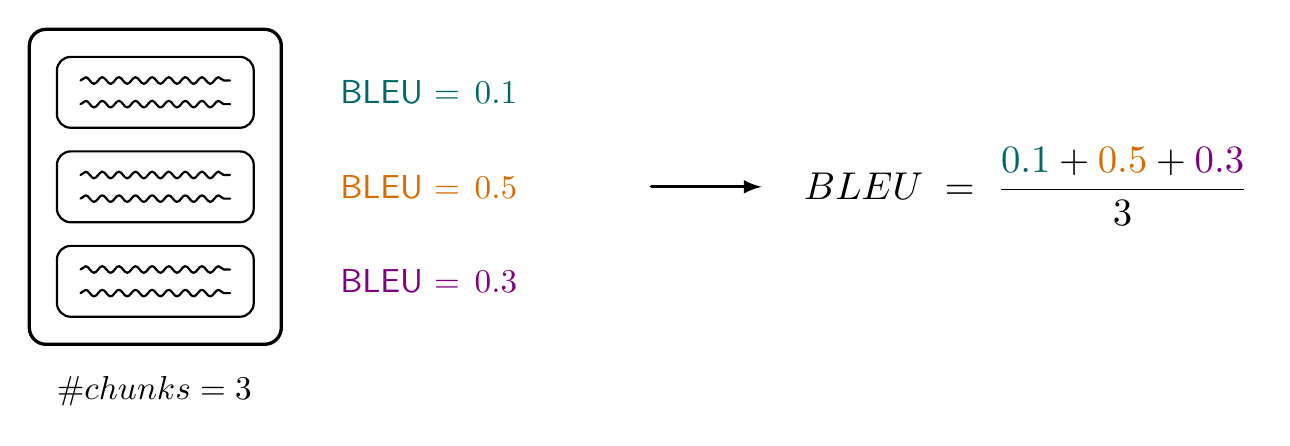
\begin{tikzpicture}[line join=round,line cap=round, >=latex, font=\sffamily]

% --- Left black container with three chunks ---
\draw[black, very thick, rounded corners=6pt]
  (-0.2,3.6) rectangle (3.0,-0.4);

% three inner rounded rectangles
\foreach \y in {2.8,1.6,0.4}{
  \draw[black, thick, rounded corners=5pt] (0.15,\y+0.45) rectangle (2.65,\y-0.45);
  % squiggle inside
  \draw[black, thick, decorate, decoration={snake,amplitude=1.2pt,segment length=6pt}]
    (0.45,\y-0.15) -- (2.35,\y-0.15);
  \draw[black, thick, decorate, decoration={snake,amplitude=1.2pt,segment length=6pt}]
  (0.45,\y+0.15) -- (2.35,\y+0.15);
}

% --- Colored BLEU labels next to each chunk ---
\node[anchor=west, text=teal!80!black, scale=1.2]  at (3.6,2.8) {BLEU $=\,0.1$};
\node[anchor=west, text=orange!85!black, scale=1.2] at (3.6,1.6) {BLEU $=\,0.5$};
\node[anchor=west, text=violet, scale=1.2]         at (3.6,0.4) {BLEU $=\,0.3$};

% --- n_chunks = 3 (black) ---
\node[anchor=west, text=black, scale=1.2] at (0.0,-1.0) {$\#\text{ chunks}=3$};

% --- Arrow to the right and mean BLEU expression ---
\draw[black, very thick, ->, >=latex] (7.7,1.6) -- (9.1,1.6);

\node[anchor=west, text=black, scale=1.4] at (9.3,1.6)
  {$\varnothing\ \text{BLEU} \;=\; \displaystyle
   \frac{\textcolor{teal!80!black}{0.1}+\textcolor{orange!85!black}{0.5}+\textcolor{violet}{0.3}}{3}$};

\end{tikzpicture}
}
  \caption[Computation of the mean \ac{bleu} score over chunks]{Computation of the mean \ac{bleu} score over three text chunks of a text.}
  \label{fig:mean-bleu}
\end{figure}


\subsection{Exp.\ 3: Assessing the Impact of the Prompt on Paraphrasing}
\label{subsec:prompt_impact}

The goal of this experiment was to investigate how different prompting strategies influence the quality of paraphrases generated by \acp{lm}.  
Since the \impAppr{} relies on paraphrased text as a basis for further computation, it is crucial to ensure that these paraphrases are both faithful to the original content and of comparable length to their references.  
Substantial deviations in length may introduce confounding factors, thereby reducing the reliability of subsequent analyses.  

We designed three prompt variants to instruct models in the paraphrasing task.
Prompt0 directs the model to paraphrase by substituting the main subject, verb, and object with synonyms, keeping the output close in length to the reference.  
Prompt1 requests a paraphrase that varies wording and sentence structure while preserving tone, with length similar to the original.  
Prompt2 instructs the model to produce a paraphrase three times longer than the reference, while preserving meaning and tone. 

We applied these prompts to the four autoregressive \acp{lm}. 
We opted for causal models since their architecture is beneficial for text generation compared to masked models.
The models include \texttt{meta-llama\-3.1-8b-instruct}, \texttt{mistral-large-instruct}, \texttt{openai-gpt-\-oss\-120b}, and \texttt{qwen3-32b}.  
You may find more details about their architecture in the in \autoref{app:language_models}.
For each model–prompt pair, we generated paraphrases of reference texts drawn from our dataset.  

% During initial exploration, we observed that some models, particularly \texttt{qwen3-32b}, produced reasoning traces, i.e.\ intermediate thought-like text segments separated by \texttt{</think>}.  
% As these traces are not part of the intended paraphrase, they were systematically removed through post-processing prior to evaluation.  

The evaluation focused on two dimensions.
Length fidelity calculates the relative difference in length between reference and paraphrase, used as a proxy for structural comparability.  
Content quality is a manual inspection of paraphrases with lengths longer and close to their references, to verify semantic preservation and readability.  

This experiment was designed to answer two key questions:  
\begin{enumerate}
    \item How strongly does the choice of prompt affect the relative length of generated paraphrases across different \acp{lm}?  
    \item Which prompt formulation best balances structural comparability and semantic fidelity, thereby reducing confounding factors for subsequent \imp{} experiments?  
\end{enumerate}


% \subsection{Exp.\ 4: Impact of Syntactic Similarity on \impApprTitle{} Effectivity}
\label{sec:syn_sim_impact_}

We designed this experiment in order to assess whether the syntactic similarity of generated paraphrases, i.e.\ the difficulty of hard negatives, influences the effectiveness of the \impAppr{}.
We conducted this experiment on both the \dataBlog{} and \dataStudent{} datasets, selecting 15~samples each from the training and test splits. 
The detector was configured according to Table~\ref{tab:imp_syn_sim_config}.

\begin{table}[h]
\centering\small
\caption{Exp.\ 4: \impAppr{} configuration.}
\label{tab:imp_syn_sim_config}
\begin{tabular}{@{}rlrrl@{}}   % numbers should be right aligned, text left aligned
\toprule
\# Impostors & Generation & Rounds & Top $n$ & Upsample \\
\midrule
50 & LLM & 100 & \num{100000} & False \\
\bottomrule
\end{tabular}%
\end{table}

For generation, we loop through all \ac{llm}-based paraphrasers until we successfully created 50~\imps{}.
One-step paraphrasers are used with both prompts.
Predictions on the test set were obtained by thresholding the detector’s scores with a decision threshold was determined using Youden’s J statistic on the training set.
We computed the average syntactic similarity on the test set. 
Following \citet{gohsen_captions_2023}, we define average syntactic similarity $\diameter_{syn}$ as the mean of the \ac{bleu}, \ac{rouge}-1, and \ac{rouge}-L scores. 
For each input pair in the test set, we calculated
(1) the average syntactic similarity between the two texts in the pair, (2) the mean average syntactic similarity between the candidate reference text and its paraphrases, and (3) the mean average syntactic similarity between the disputed text and the paraphrases.

We further grouped samples based on (1), (2), (3) and the difference (2)–(1). 
For each group, we computed accuracy, precision, recall, and F1 score of the detector’s predictions. 
The average values for each metric in a bin are presented in a bar chart.



% \subsection{Exp. 5: Comparing \acs{av} methods in traditional Human-Human scenario}
\label{subsec:imp_gen}

We want to answer the question of how our \ac{llm}-based \imp{} generation performs compared to (a) traditional \imp{} generation in the \impAppr{}~\citep{koppel_determining_2014}, and compared to (b) \ac{sota} \ac{av} methods in the traditional \ac{av} scenario.
We thus, create 100 same- and 100 different-author pairs from the \dataStudent{} 
% 1 each on and the \dataBlog{} datasets % 1 for Blog, 100 for Student Essays
dataset and evaluate the performance of the approaches for different thresholds.
It is noteworthy, that the dataset contains equally many naive same- and different-author pairs and hence, an approach predicting only one output will obtain an accuracy of $0.5$.
The \impAppr{} and unmasking detector configuration are shown in \autoref{tab:exp5_imp_config} and \autoref{tab:exp5_unmasking_config}, respectively.

\begin{table}[h]
\centering\small
\caption{Exp. 5: \impAppr{} configurations.}
\label{tab:exp5_imp_config}
\begin{tabular}{@{}rlrrl@{}}   % numbers should be right aligned, text left aligned
\toprule
\# Impostors & Generation & Rounds & Top $n$ & Upsample \\
\midrule
50 & \textit{Variable} & 100 & \num{100000} & False \\
\bottomrule
\end{tabular}%
\end{table}

\begin{table}[h]
\centering\small
\caption{Exp. 5: Unmasking configurations.}
\label{tab:exp5_unmasking_config}
\begin{tabular}{@{}rrrrl@{}}   % numbers should be right aligned, text left aligned
\toprule
\# CV Folds & \# Chunks & Rounds & Top $n$ & Upsample \\
\midrule
3 & 60 & 30 & \num{250} & False \\
\bottomrule
\end{tabular}%
\end{table}

For each impostor generation method, we computed accuracy, precision, recall, and F1 score for different thresholds. 


% \subsection{Exp. 6: Comparing \ac{av} Methods in \acs{llm} author scenarios}

This experiment evaluates the performance of the \impAppr{} in comparison to established \ac{av} methods.
As baselines, we employ generalized unmasking~\citep{bevendorff_generalizing_2019} and the compression-based approach PPMD approach and baselines from the original work~\citep{koppel_determining_2014}.
Different to experiment 5, each input pair contains at least one \ac{llm} generated text.
We compare three scenarios.
The first one simulates \ac{llm} detection, i.e. output true if the disputed text is generated by an \ac{llm}.
We design our dataset, such that candidate texts are \ac{llm} generated and the disputed texts can be either \ac{llm} generated or human authored.
A pair receives the truth label if the disputed text is \ac{llm} generated irrespective of the model used.
The second group is a \ac{llm} \ac{av} scenario where the dataset is the same as the one before, but we only label same author pairs with true.
The third scenario contains only \ac{llm} generated texts.
We denote this a more difficult \ac{llm} \ac{av} scenario.


Following the experimental setup described in \autoref{tab:av_comp} and \autoref{tab:exp6_unmasking_config} for the \impAppr{} and unmasking respectively, we assess performance using  accuracy, precision, recall, and the F1 score. 

\begin{table}[h]
\centering\small
\caption{Exp. 6: \impAppr{} configurations.}
\label{tab:av_comp}
\begin{tabular}{@{}rlrrl@{}}   % numbers should be right aligned, text left aligned
\toprule
\# Impostors & Generation & Rounds & Top $n$ & Upsample \\
\midrule
50 & \textit{Variable} & 100 & \num{100000} & False \\
\bottomrule
\end{tabular}%
\end{table}

\begin{table}[h]
\centering\small
\caption{Exp. 6: Unmasking configurations.}
\label{tab:exp6_unmasking_config}
\begin{tabular}{@{}rrrrl@{}}   % numbers should be right aligned, text left aligned
\toprule
\# CV Folds & \# Chunks & Rounds & Top $n$ & Upsample \\
\midrule
3 & 60 & 30 & \num{250} & False \\
\bottomrule
\end{tabular}%
\end{table}

\subsection{Exp.\ 5: Comparing Authorship Verification Methods}
\label{subsec:imp_gen_setup}

This experiment aims to evaluate the performance of our \ac{llm}-based \impAppr{} relative to other \ac{av} methods.
For the \ac{llm}-based \impAppr{}, we use one-step paraphrasers instructed with \texttt{prompt2} as the \imp{} generation strategy.
The experiment compares the \ac{llm}-based \impAppr{} with the traditional \impAppr{} using the \texttt{fixed} \imp{} selection strategy, the original baselines reported by \citet{koppel_determining_2014}, \unmasking{} and \ac{ppmd}. The baselines comprise unsupervised min-max similarity, unsupervised cosine similarity, and a supervised linear \ac{svm}. The supervised baseline was trained on a separate dataset to prevent any information leakage into the test results.

We sampled 20 same-author and 20 different-author text pairs from the \dataStudent{} dataset. 
Detector configurations for the \impAppr{} and \unmasking{} methods are detailed in \Cref{tab:exp5_imp_config} and \Cref{tab:exp5_unmasking_config}, respectively. 
For each \ac{av} method, we computed precision and recall across multiple thresholds and report the corresponding \ac{auc} values to summarise overall performance.

\begin{table}[h]
\centering\small
\caption{Exp.\ 5: \impAppr{} configurations.}
\label{tab:exp5_imp_config}
\begin{tabular}{@{}rlrrl@{}}   % numbers should be right aligned, text left aligned
\toprule
\# Impostors & Generation & Rounds & Top $n$ & Upsample \\
\midrule
50 & \textit{Variable} & 100 & \num{100000} & False \\
\bottomrule
\end{tabular}%
\end{table}

\begin{table}[h]
\centering\small
\caption[Exp.\ 5: Unmasking configurations]{Exp.\ 5: Unmasking configurations. CV denotes cross-validation.}
\label{tab:exp5_unmasking_config}
\begin{tabular}{@{}rrrrl@{}}   % numbers should be right aligned, text left aligned
\toprule
\# CV Folds & \# Chunks & Rounds & Top $n$ & Upsample \\
\midrule
3 & 60 & 30 & \num{250} & False \\
\bottomrule
\end{tabular}%
\end{table}








